\section{Introduction}
\label{sec:introduction}
From the Internet of Things (IoT) to the Internet of Everything (IoE), the 
common denominator is \emph{connectivity} driven by ubiquitous embedded 
systems. The goal of these devices and infrastructures is to build a 
cyber-physical framework that predicts and automates the mundane, enabling 
people to concentrate on more productive and creative things 
\cite{weldon2016future}. This digital infrastructure puts sensors on everything 
(animate and inanimate), links the sensors, does data analysis on the 
information generated by these \emph{things} to create a knowledge-base, makes 
predictions based on the available information and if it detects an anomaly, 
may take corrective, preventive or stabilizing action on the system 
\cite{ezeme2015multi}. In this way, it produces a new utility in the form of 
time which is a positive aspect. On the downside, this increased connectivity 
era implies that an automated system handles both our safety and non-safety 
critical data and actions, and a breach in the intended behavior of the 
connected devices could prove catastrophic as they manage our daily activities 
from medicine to autonomous vehicles, avionics and power systems. For embedded 
systems which are characterized by their bespoke nature and constrained 
compute and energy resources, this era of increased connectivity increases 
their vulnerability. Hence, the need to in addition to their primary functional 
requirement, they are expected to run other security and safety control models 
to maintain the integrity of their operations. This extra requirement means 
that the embedded devices have to split their available resources to satisfy 
both the primary objective and the anomaly model. While some of the systems may 
not require online anomaly monitoring due to the low-risk level associated with 
their operations, some others that perform critical tasks within a constrained 
time window require a constant update on the integrity of its operation. Hence, 
the need for an online anomaly model that can be integrated into these devices 
to monitor the conformity of the behavior of the devices with the prescribed 
operational standards. To optimize the impact of the anomaly model on the 
performance of the device 
with respect to its primary objective, we introduce a design mechanism that 
leverages the hub/edge/cloud resources to ensure that the embedded devices 
satisfy both the demands of their primary duty and that of the anomaly model. 
\par  
If the behavior of the embedded devices and their applications are 
well-characterized, then the state transition checks espoused by the authors in 
\cite{sumner2013comparative,li2017locating} can be applied to detect the 
anomalies. However, there are two challenges associated with this method of 
anomaly detection in this era of data and connectivity explosion; 
\begin{enumerate*}[label={\alph*)},font={\bfseries}]
	\item it is daunting to define all the possible states of the tuples 
	associated with a particular process running in the embedded system because 
	of the increasing complexity of tasks performed by these processes.
	\item the increasing complexity of the functions \cite{ezeme2015multi} 
	performed by these cyber-physical embedded systems demands a high level of 
	dynamism which makes the use of static state transition analysis untenable.
\end{enumerate*}  
Therefore, we propose a \emph{dynamic, distributed} and \emph{self-scaling} 
anomaly detection model that utilizes the temporal information in the system 
call execution sequences to detect anomalies. 
\par  
The anomaly model processes the traces as streams of tuples and takes into 
account the temporal drift by building a profile that can create both short and 
long-term contexts of the sequences. The use of the LSTM cells and 
context-based attention layer provides medium to short-term contexts while the 
incorporation of the feedback input from the attention layer creates a 
long-range dependency between the present and past inputs to the model. This 
dynamic approach enables us to target both previously known and unknown 
anomalies and deepens the understanding of the execution contexts of the kernel 
events \emph{horizontally} and \emph{vertically}. This overall design employs 
the concept of transfer learning 
as we start with an unsupervised prediction model and use the knowledge from 
the unsupervised learning phase to create a fast supervised classifier to 
detect when an anomaly has occurred. The training employs a closed-world 
approach; hence only the kernel events from the standard operating profiles are 
used for training the unsupervised model.  \par
To facilitate the capture of long and short-term temporal dependencies, we use 
a stack of the Long Short-Term Memory (LSTM) \cite{hochreiter1997long} which 
its variants have been used in various tasks to demonstrate its effectiveness 
in capturing complex non-linear relationships that exist in a sequence. The use 
of hierarchical LSTM learns the temporal relationships amongst events while the 
attention layer determines in small details, the impact of each feature in one 
another. This strategy helps to filter out the effect of the randomness 
prevalent in kernel events as a result of interrupts. Our anomaly model uses a 
context-aware variant of the attention mechanism which does three functions; 
\begin{enumerate*}[label={\alph*)},font={\bfseries}]
	\item within tuples in a window under consideration, it improves the target 
	tuple prediction accuracy by diminishing the effect of unessential source 
	inputs for any target output.
	\item it narrows the dimension of the hidden state output of the LSTM and 
	introduces flexibility in handling the size of the output vector.
	\item between predictions, the attention layer controls the influence of 
	the previous output on the next target by forming a component of the 
	context vector that controls the alignment of the next prediction.
\end{enumerate*}
And this helps to answer the \emph{why} question in the 
computation of the prediction by giving us a view of the \emph{features} that 
influence each output. The logic in 
our reasoning is that just like natural language, each tuple has different 
contexts based on usage and the effect of the present tuple $ \bm{V_t} $ on 
next 
prediction $ \bm{V_{t+1}} $ should be derived from a deeper and longer context 
than 
just the present tuple $ \bm{V_t} $ and the present attention vector $ \bm{Z_t} 
$ because concurrently running tasks can make the order of the traces complex 
to analyze. 
Therefore, in comparison with other design architectures, our design varies on 
how the context vector is constructed and used in both the attention layer and 
next target prediction. And this is one of the principal technical 
contributions of the work. \par
The primary target of the work is system logs from operating systems like 
kernel events or system calls. To handle bias in the model, in each layer of 
the system which generates the logs, we train the model only 
with attributes that cut across the different formats emitted by the different 
kinds of operating systems for the layer under consideration. Example of the 
characteristics of system calls sequence is $\text{open} \longrightarrow
\text{mmap} \longrightarrow \text{read} \longrightarrow \text{close}$ and 
these are used as features to train the model and get the classifier for this 
layer. Therefore, we have two problem statements as thus: 
\begin{enumerate*}[label={\alph*)},font={\bfseries}]
	\item given kernel events obtained during the normal operation of a system, 
	is it possible to create a model that uses the information solely from 
	normal behavior to characterize the standard and deviant behaviors in the 
	kernel events?
	\item if yes, can we dynamically deploy this anomaly model to perform 
	online anomaly detection by leveraging hub/edge/cloud resources?
\end{enumerate*}
To answer the questions posed above, we propose a \emph{distributed and 
self-scaling anomaly detection model} primarily targeting resource-constrained 
embedded systems. In summary, our contributions are:
\begin{enumerate*}[label={\alph*)},font={\bfseries}]
	\item we present a dynamic, distributed and self-scaling mechanism to 
	leverage hub/edge/cloud resources to complement the operation of an 
	embedded system.
	\item we present an online deep context-aware architecture for anomaly 
	detection in semi-structured sequences with bias to kernel events.
\end{enumerate*} \par
To ease the comprehension of the work, we have divided the rest of the work 
into the following sections; Section \ref{sec:related-work} briefly highlights 
the related work in this domain. Section \ref{sec:design} discusses the 
technical details of our model while Section \ref{sec:experiments} details our 
tests as well as discussion of the results. In Section \ref{sec:conclusion}, we 
conclude the work with an insight into our prospective research directions.

\section{Related Work}
\label{sec:related-work}
According to \cite{chandola2009anomaly}, the two broad categories of detecting 
deviant behavior during system operation are \emph{intrusion} and 
\emph{anomaly} detection. While both techniques can detect previously seen 
anomalies, only the anomaly method monitors both known and unknown deviation 
from the standard performance behavior. The use of \emph{models} instead of 
\emph{signatures} enhances the capability of the anomaly method to track 
\emph{zero-day} vulnerabilities. The intrusion (signature) method has extensive 
details in \cite{garcia2009anomaly}. The obvious limitation of this 
signature-based method is that \emph{zero-day} vulnerabilities cannot be 
detected as it only searches for known signatures. On the other hand, authors 
in \cite{Ezeme2017,du2017deeplog,xu2009largescale,yu2016cloudseer} use the 
anomaly-based approach which involves the construction of a model to target 
both known and unknown aberrations. This model-based technique comes at the 
cost of doing \emph{feature extraction} from the operational profiles, 
\emph{processing} the extracted features to conform to the model input 
requirements, and finally, model design and training with the profile features. 
While this method provides versatility in terms of its target threat domain, it 
has higher false positives than the signature-based intrusion detection 
mechanisms.\par 
In \cite{Ezeme2017}, the authors explored the use of a vector space model with 
hierarchical clustering that creates a binary profile to determine if an 
observed profile sequences are anomalous or not. While this model shows an 
excellent result in the experiments used by the authors, its scalability is 
limited because of the enormous number of tuples it needs to make a decision. 
Authors of \cite{yoon2017learning} also have a vector space model based anomaly 
detection method which categories system processes using their system call 
information. This model suffers from the same scalability issue as that of 
\cite{Ezeme2017} because it requires a long window of observation before it can 
make a decision. The authors of \cite{du2017deeplog} built an anomaly detection 
framework called \emph{Deeplog} using two layers of LSTM networks and a 
workflow construction approach for each 
key in the log for diagnostics. This \emph{Deeplog} framework uses LSTM also, 
but there is no notion of attention layer in the framework. Also, the authors 
of \cite{gu2005detecting} used the statistical metric of entropy to implement 
an anomaly detection model for network logs but this type of anomaly model is 
best suited for cases where the volume of logs determine if an anomaly has 
occurred as obtainable in denial of service attack. In 
\cite{salem2016anomaly}, a real-time systems anomaly detection model is 
designed using the principle of inter-arrival curves to detect anomalous traces 
in a log sequence. However, this inter-arrival curve-based model works offline 
because it requires a large number of logs before it computes the curves. 
Reference \cite{xu2009largescale} designed a vector space model to mine console 
logs for anomalies and \cite{li2017locating} used an optimization method of 
minimum debugging frontier sets to create a model for detection of 
errors/faults in software execution. In \cite{Ezeme2018RTCSA}, the authors use 
the kernel event tuples to design an anomaly model based on the concept of the 
encoder-decoder approach. It uses an attention layer to aid in sequence 
reconstruction at the prediction phase. Although this approach is close to our 
method, we differ both in the model architecture and target platform. 
Therefore, while we introduce design mechanism to ensure a truly dynamic and 
distributed anomaly model, \cite{Ezeme2018RTCSA} creates a centralized anomaly 
model that places a considerable strain on embedded system resources, thereby 
limiting its use for online anomaly detection.

\section{Model Architecture}
\label{sec:design}
Fig. \ref{fig:distributed-architecture} is the design of our distributed model 
that provides the three core features of \emph{dynamism, self-scalability} and 
\emph{distribution} of the anomaly model amongst the local and cloud resources. 
The break down of the modules of Fig. \ref{fig:distributed-architecture} is 
discussed in the sub-sections below. Also, we have broadly broken down the 
actual anomaly detection model of Fig. \ref{fig:deep-model} into two modules 
identified in the figure as \emph{predictor} and \emph{detector}. Before we 
proceed further, it is important that we explain some of the names in Fig. 
\ref{fig:distributed-architecture}. \emph{PUSH, PULL, PUB,} and \emph{SUB} are 
ZeroMQ TCP sockets while \emph{STAGES} $ 1 $ and $ 2 $ represent the points 
where distribution decisions are taken. We use ZeroMQ sockets in our design 
because unlike the traditional TCP sockets available in the operating system, 
ZeroMQ sockets pairs can be connected and disconnected arbitrarily in no 
particular order. This arbitrary connection and disconnection ability removes 
the need of restarting the system if one of the pairs dies and tries to 
reconnect. We discuss the different modules of Fig. 
\ref{fig:distributed-architecture} in the sub-sections below.
\begin{figure}[!t]
	\centering
	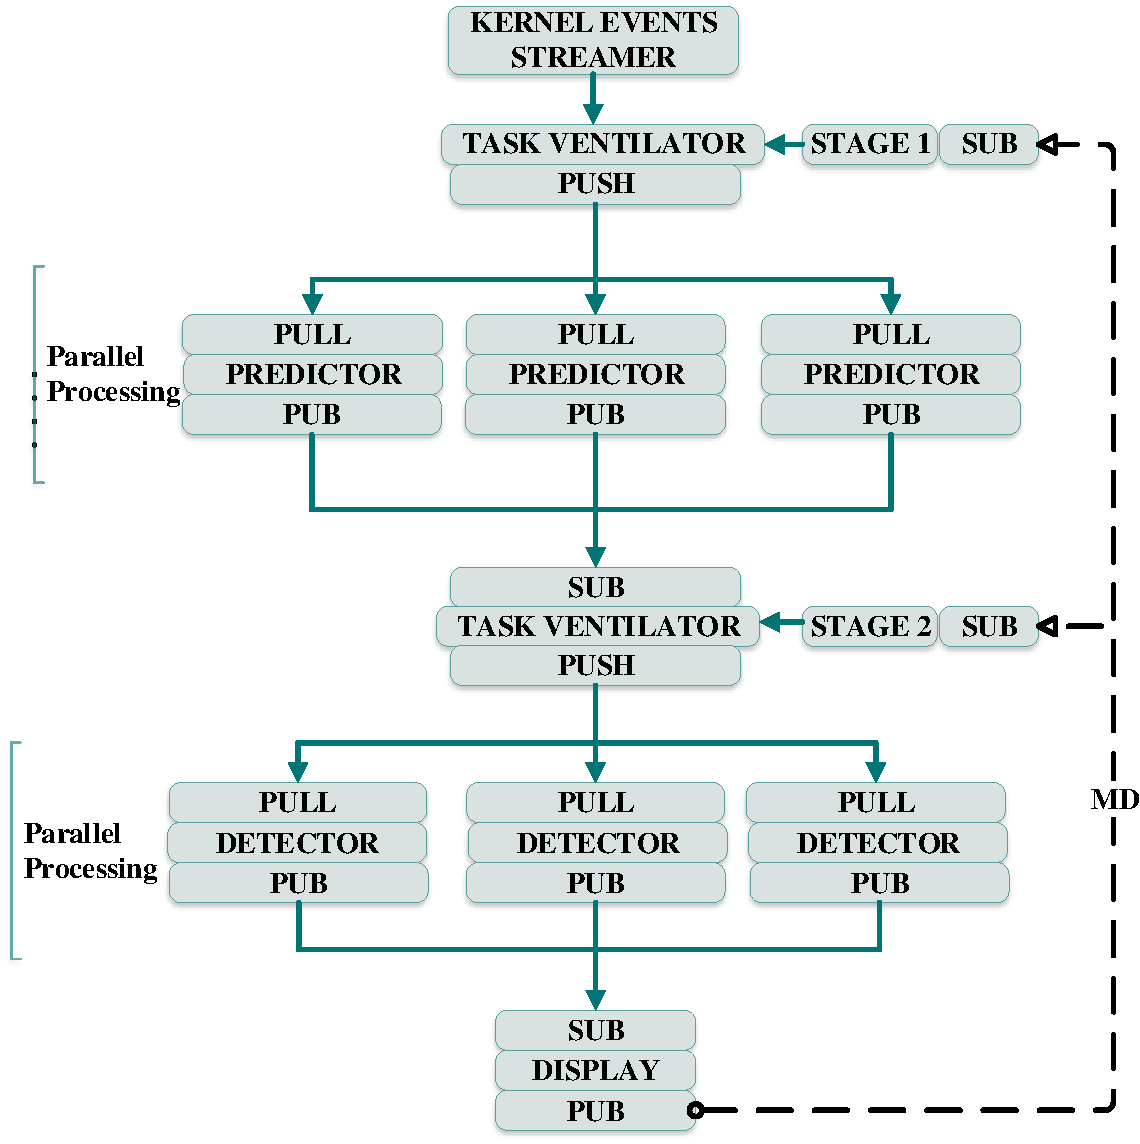
\includegraphics[scale=0.45]{decomposed-model.pdf}
	\caption{Dynamic, Distributed and Self-Scaling Architecture for Anomaly 
	Model Deployment}
	\label{fig:distributed-architecture}
\end{figure}


\begin{figure}[!t]
	\centering
	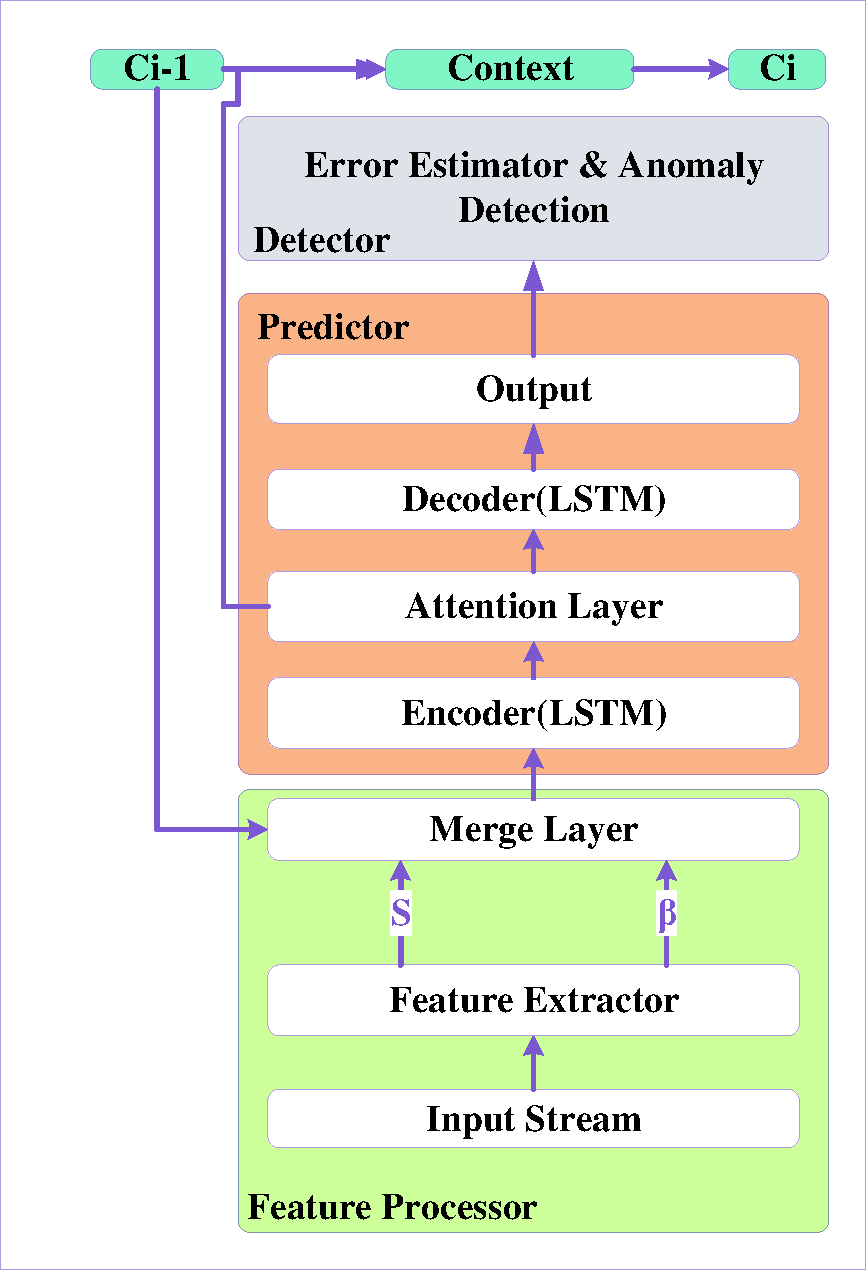
\includegraphics[scale=0.45]{anomaly-model.pdf} 
	\caption{A Recursive Deep Context Anomaly Detection Model 
	}
	\label{fig:deep-model}
\end{figure}

\subsection{Stage 1 Ventilator Module}
\label{subsec:stage1}
\subsubsection*{Kernel Event Streamer}
\label{subsec:preprocessing}
The \emph{kernel events streamer} is a module that handles the processing of 
the kernel events emanating from the instrumented kernel. The raw kernel events 
have both useful and non-useful attributes for our model design. Therefore, the 
streamer module extracts the useful information from the kernel events and 
positions the events in the format accepted by the model. As we mentioned in 
Section \ref{sec:introduction}, we only process the attributes which are common 
across the trace irrespective of the system to remove any system-induced bias 
on the classifier. In kernel, an 
example event stream of $\text{THRUNNING} \longrightarrow \text{THREADY} 
\longrightarrow \text{THRECEIVE} \longrightarrow \text{THREPLY}$ has 
\emph{timestamps, PID, TID, NID}, etc. which are common across the event 
stream. Therefore, we formulate the characteristics of interest using these 
features which exist across kernel event streams irrespective of platform.
\subsubsection*{Task Ventilation}
\label{subsub:task1}
The frequency of the kernel event streamer is high, and the downstream modules 
have to keep up with the streams in order to avoid the sockets dropping the 
data. Hence, the need for parallelism at the \emph{predictor}. As stated in 
Section \ref{sec:design}, the sockets can connect and disconnect arbitrarily 
without restarting the network thereby providing an efficient horizontal 
scaling mechanism for the parallel predictors and detectors. Our dynamic 
allocation scheme starts in \eqref{eq:new-pred-num} where we determine the 
number of new predictors $ \bm{N_p} $ we can create locally using the free 
system resources (compute and memory) $ \bm{R_{s}} $, the energy level $ 
\bm{E_l} $ of the embedded device and the system resources $ \bm{R_p} $ 
required by a predictor. 

\begin{align}
\label{eq:new-pred-num}
\bm{N_p} &= \bm{\frac{R_{s}\times E_{l}}{R_{p}}} \\
\label{eq:total-pred-local}
\bm{\tau_{p}} &= \bm{N_p + N_{local}}
\end{align}
The total number of predictors that we can run on the embedded device is given 
in \eqref{eq:total-pred-local} pending the outcome of conditions 
\eqref{eq:PI-local} and \eqref{eq:PI-cloud}. $ \bm{N_{local}} $ of 
\eqref{eq:total-pred-local} refers to already running instances of predictors 
on the embedded device.
\begin{align}
	\label{eq:PI-local}
	\bm{PI_{local}} & = \bm{\frac{\tau_{p}}{C_p\times F_k}} \\
	\label{eq:PI-cloud}
	\bm{PI_{cloud}} &= \bm{\frac{TDD_1}{PI_{local}\times \lambda}}\; 
	\text{where} \; \lambda \ge 1
\end{align}
To determine the performance of the predictors locally and in the cloud, we use 
\eqref{eq:PI-local} and \eqref{eq:PI-cloud} which we refer to as the local 
(embedded device) and cloud performance index (PI) respectively. $ \bm{C_p} $ 
and $ 
\bm{F_k} $ refers to the computational time of the predictor in seconds and the 
kernel event streamer frequency which is measured in input/seconds. In 
\eqref{eq:PI-cloud}, $ \bm{\lambda} $ is the speed factor we get for processing 
in the cloud and $ \bm{TDD_1} $ is the total delay from the ventilator to the 
display when the predictors in the cloud are used. The metadata feedback loop 
of Fig. \ref{fig:distributed-architecture} provides the $ \bm{TDD_1} $ 
information. For every task sent to the cloud from the stage 1 ventilator, the 
cloud detector is equally used for anomaly detection and the result published 
to the display. In our model, there is no automatic system reaction to the 
detection of an anomaly; hence we envisage the display to be operated by a 
human operator. Therefore, the display is assumed to be in the monitoring room. 
The SUB sockets of the stage 2 task ventilator and the display provide the 
metadata information on the number of parallel predictors and detectors running 
locally via the metadata (MD) feedback loop.
Now, examining \eqref{eq:PI-local} and \eqref{eq:PI-cloud} closely, we see that 
they vary inversely to one another. So, as the streaming frequency $ \bm{F_k} $ 
increases compared to the available number of predictors, the local performance 
index $ \bm{PI_{local}} $ decreases and the cloud performance index $ 
\bm{PI_{cloud}} $ increases, thereby favoring more predictors to be run in the 
cloud and vice versa. Therefore, \eqref{eq:new-pred-num} to \eqref{eq:PI-cloud} 
create a \emph{self-scalable} and \emph{distributed} system for handling both 
the predictor and detector tasks. The latency requirement of the application 
places a bound on the viable values of $ \bm{TDD_1} $ that is permissible in 
the model.

\subsection{Predictor}
\label{subsec:predictor}
\subsubsection*{Merge Layer}
Our hypothesis is based on creating a deep execution context via a recursive 
input generated from the attention layer. Since the attention layer has a 
learned weight, it means that its output which is used to create the context $ 
C $ contains information of multiple previous inputs, and feeding it along with 
the present input either reinforces a standard profile or weakens the 
prediction accuracy which will indicate the presence of an anomaly. Therefore, 
\eqref{eq:merge-out} describes our approach of merging the recursive input $ 
\bm{C_i} $ with the present input $ \bm{X_i} $.
\begin{equation}
\bm{v} = \text{merge}(\bm{\vec{X_i},\vec{C_i}}) \\
\label{eq:merge-out}
\end{equation}

\subsubsection*{Encoder (LSTM Layer)}
\label{subsubsec:encoder}
Our choice of LSTM cells in this layer stems from the fact that it is designed 
primarily for time-series data and its recursive nature helps to propagate 
temporal information across so many timesteps infinitely in theory. However, we 
recognize that in practice, there is a limit to how far behind it can propagate 
the errors before the vanishing gradient problem sets in. Hence, our idea to 
augment it with a 
recursive context to improve the learnability over a long span of time. We 
feed the output of \eqref{eq:merge-out} to the LSTM layer. Different kinds of 
LSTM configuration can be used, but we use the LSTM units described in 
\cite{hochreiter1997long} to create our layer. This layer's output is captured 
mathematically in \eqref{eq:lstm-out}. We omit the bias terms for brevity, and 
$ \bm{\Phi} $ is a nonlinear function like an LSTM. 
\begin{align}
\bm{h}_{i} &= \bm{\Phi}\left(\bm{v}_i,\bm{h}_{i-1} \right)
\label{eq:lstm-out}
\end{align}

\subsubsection*{Attention Layer}
\label{subsubsec:attention}
Differing from \cite{salton2017attentive} that uses memory to create context, 
we add a query weight $\bm{W}_q$ that is learned during training to ensure that 
each tuple is not attended to solely based on the information in the present 
input sequence but also based on the knowledge gained during the learning 
phase. This query performs a similar role as the term-frequency inverse 
document frequency used to weigh the occurrence of tuples in the vector space 
model. The inputs to this layer are the 
input weights $\bm{W}_i$ and the LSTM layer output $\bm{h}_{i} $ of 
\eqref{eq:lstm-out}. We pass the LSTM layer output via a $\tanh$ layer after 
being scaled by the input weights $\bm{W}_i $ and the input bias vector $ 
\bm{b}_i $ to generate correlation vectors $ \bm{m}_i $ given in 
\eqref{eq:m-attention}.

\begin{equation}
\label{eq:m-attention}
\bm{m}_i = \tanh (\bm{W}_{i} \cdot \bm{h}_{i} + \bm{b}_i)
\end{equation}

The correlation vector \eqref{eq:m-attention} represents the effect 
of each input based on the present. Hence, we multiply it with the query 
vector $ \bm{W}_q $ which has the \emph{global knowledge} of each input tuple 
in the present input sequence to provide deep horizontally spanning inputs for 
the inference process as shown in \eqref{eq:q-vectors}. This vector is then 
passed through a softmax layer to generate $ \bm{s}_i $ in \eqref{eq:softmax}. 
This normalized value is scaled by the input vectors $ 
\bm{h}_{i}$ and summed to generate the attention vector $ \bm{Z}_i $ in 
\eqref{eq:z-context}.
\begin{align}
\bm{a}_i &= \bm{W}_{q} \cdot \bm{m}_i + \bm{b}_q \label{eq:q-vectors} \\
\bm{s}_i &= \left( \frac{e^{\bm{a}_i}}{\sum_j e^{\bm{a}_j}}\right)_i 
\label{eq:softmax} \\
\bm{Z}_i &= \sum_{i=1}^n \bm{s}_i \times \bm{h}_{i} \label{eq:z-context}
\end{align}

\subsubsection*{Decoder (LSTM Layer)}
This layer performs the function of a decoder while the lower LSTM is 
responsible for encoding the input. This layer in conjunction with the fully 
connected layer tries to reconstruct the input sequence. This layer creates an 
intermediate output $ \bm{h}_{_di} $ using the previous output $ \bm{y}_{i-1} 
$, the context vector $ \bm{Z} $ and the previous
hidden state $\bm{h}_{_di-1}$ of the previous unit $ d_{i-1} $. Equation 
\eqref{eq:decoder} defines this relationship where $ \Psi $ is a nonlinear 
function called LSTM. Again, bias vector is omitted for brevity.
\begin{align}
\bm{h}_{_di} &= \Psi\left(\bm{h}_{_di-1},\bm{y}_{i-1},\bm{Z}\right) 
\label{eq:decoder}
\end{align}

\subsubsection*{Output Layer}
\label{subsubsec:decoder}
Our output layer is a simple dense layer with same number of units as there are 
unique features in the input sequences. The output of this layer is given in 
\eqref{eq:fc-layer} where $ \bm{h}_{_di} $, $ \bm{W}_z $ and $ \bm{b}_z $ are 
the decoding LSTM layer output, the layer weight and the bias vector 
respectively. 
\begin{equation}
\label{eq:fc-layer}
\bm{y}_i = \bm{W}_{z} \cdot \bm{h}_{_di} + \bm{b}_z
\end{equation}
The $ \bm{y}_i $ is then passed through a softmax layer to produce the 
predicted system call $ \mathbf{S}_i $. 


\subsection{Stage 2 Ventilator Module}
\label{subsec:stage2}
We apply the stage 1 ventilator equations of Section \ref{subsec:stage1} to 
determine how we distribute the detectors but $ \bm{TDD_2} $ replaces $ 
\bm{TDD_1} $ and reference symbol is now the detector $ \bm{d} $ and not the 
predictor $ \bm{p} $. 
\subsection{Detector}
\label{subsec:detector}
\subsubsection*{Error Estimator and Anomaly Detection}
\label{subsec:error-model}
Given $ \bm{x}_i \in \bm{\mathbb{R}} $ which serves as the input, the target 
during learning is a shifted version $ \bm{x}_{i+w} \in \bm{\mathbb{R}} $ where 
$ \bm{w} $ is the lookahead window. Therefore, the goal is to replicate the 
sequence at the output by creating $ \bm{x}' \in \bm{\mathbb{R}}$. Hence, the 
perfect result is when $\bm{x}_k  \equiv \bm{x}'_k $, but this is hardly 
feasible because of the high randomness caused by interrupts and other events 
in the traces. Hence, when we have $ \bm{f}:\bm{x}\longmapsto \bm{x}' $ given $ 
\bm{x} $ as the ground truths, the deviation $ \bm{d} = \abs{\bm{x} - \bm{x}'} 
$ is the difference between the ground truth and the predicted value for the 
given sequence. This deviation becomes the prediction error values which we use 
to to fit a non-parametric kernel density estimator. The output of the 
estimator is clustered with k-means clustering where $ \bm{k=2} $.

\subsection{Display}
\label{subsec:display}
We send the clustering decision to the display via the PUB sockets of the 
detector. The display extracts the metadata information and relays the same to 
stages 1 and 2. Information from the display can also be used for corrective 
actions when an anomaly is detected. 


\section{Experimental Evaluation}
\label{sec:experiments}
\subsection{Dataset}
We use the publicly available kernel event dataset of \cite{salem2016anomaly} 
to test our model. According to the authors in \cite{salem2016anomaly}, the 
\emph{hilRf-InFin} scenario corresponds to the default system setting while 
\emph{full-while} scenario refers to generating fictitious tasks via a while 
loop to waste CPU resources by competing for the same CPU resource with the 
standard tasks running the UAV. The \emph{fifo-ls} and \emph{sporadic} 
situations derive their names from the scheduling algorithms in the operating 
system and are identified by the corresponding scheduling algorithm used in 
each experiment. 
\subsection{Experimental Setup and Networking}
Our testbed constitutes of Raspberry PI 3 platform which serves as our local 
embedded device and an Intel-i5 laptop which serves as our cloud. Each of the 
scenarios in the dataset has a separate model, and our 
experimental objectives are:
\begin{enumerate*}[label={\alph*)},font={\bfseries}]
	\item demonstrate the offloading mechanism which creates a self-scaling and 
	a distributed model.  
	\item demonstrate the improvement brought by the attention layer to the 
	anomaly model by comparing with a \emph{base} (no attention layer) model.
\end{enumerate*}
We implement our model of Fig. \ref{fig:distributed-architecture} using ZeroMQ 
\cite{Akgul:ZEROMQ}. First, the predictor and detector model weights are loaded 
in both the Raspberry PI and the laptop computer which serves as our 
cloud. Our sockets does not have restrictions on which end \emph{binds} and 
which end \emph{connects}. Therefore, it our design decision that any 
\emph{one-to-many} connection like that of \emph{stage 1 task ventilator PUSH} 
socket and \emph{predictor PULL} sockets, \emph{stage 2 task ventilator PUSH} 
and \emph{detector PULL} sockets, we bind the \emph{one} and connect the 
\emph{many}. This way, the PULL socket processes in the predictor and detector 
can be scaled up and down without affecting the network functionality since 
ZeroMQ permits arbitrary 
\emph{connect} and \emph{disconnect}. For the \emph{many-to-one} connection of 
the \emph{predictor PUB} and the \emph{stage 2 task ventilator SUB}, 
\emph{detector PUB} and \emph{display SUB}, we bind the \emph{one} and connect 
the \emph{many} as well. The \emph{PUSH-PULL} sockets provide 
\emph{parallelism} while the \emph{PUB-SUB} sockets act as \emph{source-sink} 
connection. The metadata \emph{MD} feedback loop implemented with a 
\emph{PUB-SUB} connection carries 
information about the active number of predictors and detectors as well as the 
$ \bm{TDD_1} 
$ and $ \bm{TDD_2} $ delay.
\subsection{Results}
\subsubsection{Offloading Mechanism Results}
To test the offloading mechanism, we vary the number of running processes in 
the Raspberry PI from nearly idle to near full utilization of the CPU and 
memory. We fixed the maximum number of predictors and detectors that can be run 
both in the cloud and the embedded device using \eqref{eq:total-pred-local}. 
Then, we allow the offloading mechanism to use the interaction between the $ 
\bm{PI_{local}} $ and $ \bm{PI_{cloud}} $ to generate the cloud and local 
performance index as the system gets busier. The number of local detectors and 
predictors running in a particular platform is directly proportional to its 
performance index $ \bm{PI} $. In Fig. \ref{fig:PI-plot}, we plot the $ \bm{PI} 
$ of the \emph{local} (embedded system) versus the \emph{cloud} platform. We 
place the Raspberry PI in the same network as the laptop and also experiment 
with both of the devices in different networks. In both cases, the patterns of 
the $ \bm{PI} $ plot is the same except for a slow rise time of the $ 
\bm{PI_{cloud}} $ when the $ \bm{TDD} $ is high due to network congestion. We 
determine the maximum $ \bm{TDD} $ based on heuristic when there is mild 
traffic in the network as $\bm{TDD}  = \bm{p_d+t_d+p_t}$  where $\bm{p_d}$ is 
the \emph{propagation 
delay}, $\bm{t_d}$ is the \emph{transmission delay} and $\bm{p_t}$ is the 
\emph{processing time} at the cloud.
\begin{figure}[!t]
	\centering
	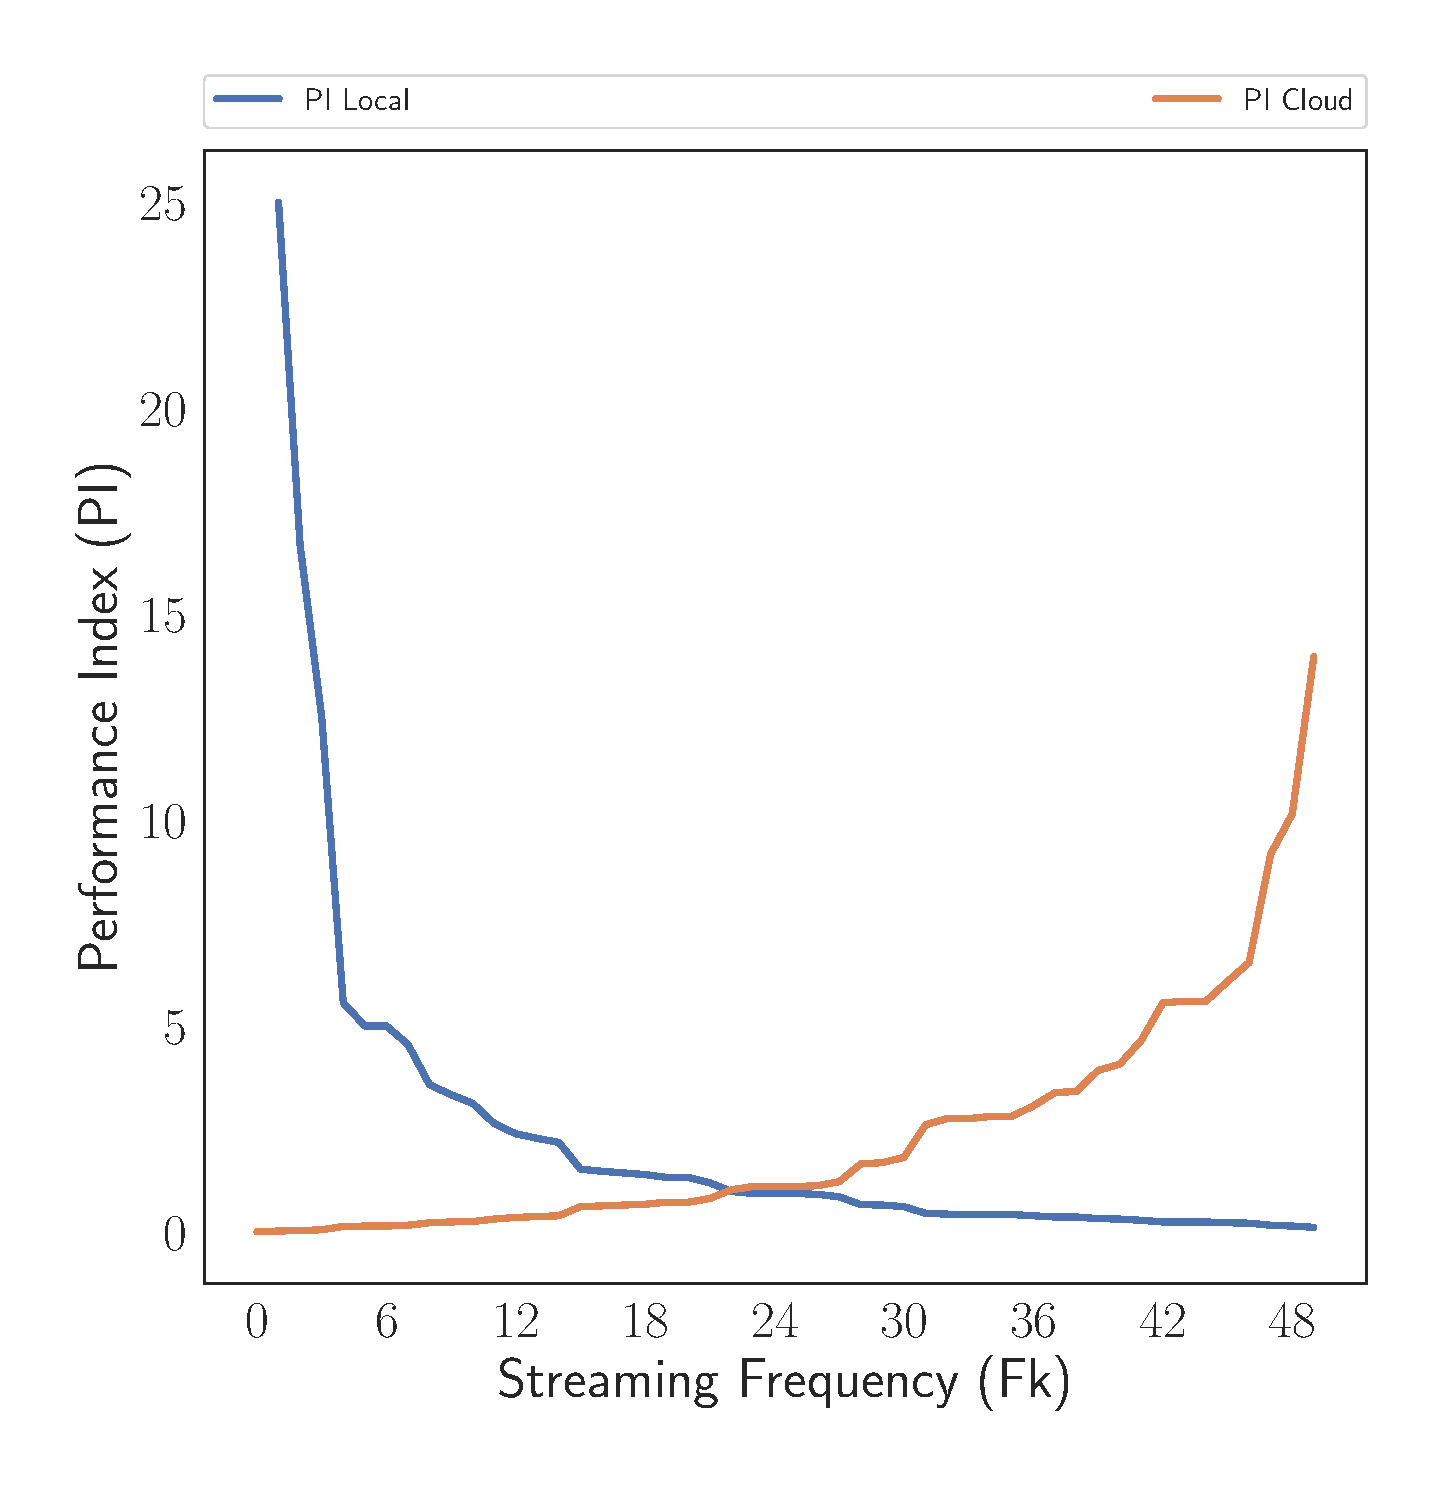
\includegraphics[scale=0.37]{performance-index.pdf} 
	\caption{Performance Index $ \bm{PI} $ of the Cloud and Embedded (Local)  
	Platform versus Streaming Frequency $ \bm{F_k} $}
	\label{fig:PI-plot}
\end{figure}
\begin{table}[!t]
	\renewcommand{\arraystretch}{1}
	\caption{Accuracy of Attention-Based Model vs the Base Model with Varying $ 
	\bm{\Phi_i} $}
	\label{tab:model-results}
	\centering
	\begin{tabu} to 0.49\textwidth {|X[l]|X[c]|X[c]|X[c]|X[c]|}
		\hline
		Experiment & Models & \multicolumn{3}{|c|}{Lookahead Window Accuracy} \\
		\hline
		& &$ \Phi_{1} $&$ \Phi_{5} $&$ \Phi_{10} $ \\
		\cline{1-5}
		\multirow{3}{*}{fifo} & Base & $ 0.794 $ & $ 0.746 $ & $ 0.724 $ \\
		\cline{2-5}
		& Att-Model & $ 0.981 $ & $ 0.972 $ & $ 0.947 $ \\
		\hline 
		\multirow{2}{*}{full}& Base & $ 0.836 $ & $ 0.791 $ & $ 0.767 $ \\
		\cline{2-5}
		& Att-Model & $ 0.99 $ & $ 0.942 $ & $ 0.916 $  \\
		\hline 
		\multirow{2}{*}{hilrf}& Base & $ 0.870 $ & $ 0.815 $ & $ 0.778 $ \\
		\cline{2-5}
		& Att-Model & $ 0.968 $ & $ 0.937 $ & $ 0.908 $ \\
		\hline
		\multirow{2}{*}{sporadic}& Base & $ 0.790 $ & $ 0.772 $ & $ 0.728 $  \\
		\cline{2-5}
		& Att-Model & $ 0.916 $ & $ 0.872 $ & $ 0.857 $ \\
		\hline 
	\end{tabu}
\end{table}
\subsubsection{Base Model vs Attention-based Model Results}
\label{subsec:att-vs-noatt}
With high input frequency rate, we varied the lookahead window to reduce the 
number of iterations that we run the predictor and the detector and conserve 
the embedded system resources. While this conserves resources, its 
effectiveness depends on the accuracy of our model. We represent the ratio of 
the input stream window to the output lookahead window as $ \bm{\Phi} = 
\nicefrac{\theta_{in}}{\theta_{out}} $. Therefore, $ \bm{\Phi_{i}} $ is the 
\emph{input-output} window ratio for lookahead length $ \bm{i} $. We use early 
stopping and dynamic learning rate during training to control the number of 
training epochs and improve the performance of the \emph{adam} 
\cite{kingma2014adam} optimization scheme that was used during the training 
process. In Table \ref{tab:model-results}, two patterns emerge:
\begin{enumerate*}[label={\alph*)},font={\bfseries}]
	\item the attention-based model we designed consistently outperforms the 
	base model in every $ \bm{\Phi_i} 
	$.
	\item there is decreasing accuracy as we increase $ \bm{i} $ in $ \bm{\Phi} 
	$. 
\end{enumerate*}
These patterns conform with our postulation that the attention layer and the 
recursive input of of the model impact positively on the model performance. 
Also, with a fixed input window, $ \theta_{in} $, the decreasing accuracy with 
increasing $ \theta_{out} $ is expected as the temporal information needed for 
longer sequence generation is restricted.

\section{Conclusions and Future Work}
\label{sec:conclusion}
We propose a dynamic, distributed and self-scaling anomaly detection model 
targeting resource-constrained embedded devices. We detail the implementation 
of the model as well as the hypothesis behind the model design. Our 
experimental results validate our hypothesis on the offloading scheme. Also, 
the postulation of creating a recursive-context using the attention layer is 
confirmed as shown in the results. Finally, while our model can be deployed for 
\emph{soft} real-time systems, we will be exploring more robust offloading 
schemes for \emph{hard} real-time embedded applications so that the $ TDD $ 
bounds are based on real-time application's latency requirement.